\documentclass[10pt,conference]{IEEEtran}

\usepackage{array}
\usepackage{url}
\usepackage{float}
\usepackage{booktabs}
\usepackage{graphicx}
\usepackage{xcolor}
\usepackage{tikz}
\usetikzlibrary{arrows.meta,positioning}
\setlength{\textfloatsep}{6pt}
\setlength{\floatsep}{5pt}
\setlength{\intextsep}{5pt}
\renewcommand{\arraystretch}{1.0}

\title{An End-to-End Demonstration System for AI-Generated Talking-Head Content in Social-Media Scam Awareness and Prevention}

\author{\IEEEauthorblockN{Alice / Xinran Yang}
\IEEEauthorblockA{AI Project Proposal Draft}}

\begin{document}
\maketitle

\begin{abstract}
The rise of AI tools has made identity shifting increasingly easy, allowing attackers to impersonate real people through synthesised faces and voices, thus raising new risks of social-media scams. This project develops a system that shows how such deceptive content can be produced, thus raising public awareness and supporting prevention strategies. This system will combine a voice conversion model with an audio-driven talking-head model to generate synthesised video content from a static facial image and a target voice sample. The final system is designed to automatically collect facial and voice information from publicly available social-media content and use this material to generate a talking-head video that simulates a realistic scam scenario. The demonstration aims to improve awareness of AI-driven identity shifting and support discussion of possible countermeasures such as user education and content verification.
\end{abstract}

\begin{IEEEkeywords}
talking-head generation, voice cloning, social-media scams, synthetic media, scam awareness, responsible AI
\end{IEEEkeywords}

\section{Background}
AI-generated identity shifting is becoming easier for non-expert users. A convincing scam message no longer needs only text: an attacker may combine a public profile image, a short voice sample, and a generated script to create a video that appears to come from a trusted person. This raises risks for social-media users, especially when people rely on familiar faces and voices as trust signals.

This project addresses that risk through a controlled demonstration system. The purpose is not to create a tool for deception, but to show how the attack pipeline can work, evaluate where the technology succeeds or fails, and use the evidence to support awareness and prevention. The project therefore has two connected goals: building an end-to-end technical prototype and analysing the conditions under which the output becomes convincing, fragile, or clearly synthetic.

Existing talking-head systems provide useful components but do not, by themselves, answer the project question. Wav2Lip focuses on lip synchronization~\cite{wav2lip}; Audio2Head represents audio-driven one-shot talking-head generation with natural head motion~\cite{audio2head}; SadTalker uses 3D motion coefficients for single-image animation~\cite{sadtalker}; EchoMimic provides a diffusion-style portrait-animation baseline~\cite{echomimic}; MuseTalk uses latent-space inpainting for high-quality mouth motion~\cite{musetalk}; and Chatterbox provides text-to-speech and voice-cloning capability~\cite{chatterbox}. The project compares Audio2Head, SadTalker, EchoMimic, and MuseTalk on an identity-balanced HDTF-80$\times$12 setting and uses this four-generator comparison as the technical evaluation foundation for the social-media scam-awareness workflow, including data provenance, consent limits, comparison experiments, and failure analysis.

\section{Original Contribution and Use of AI Tools}
The project separates student-led design and implementation work from AI systems and existing open-source tools. Table~\ref{tab:own_ai} separates these roles.

\begin{table}[H]
\caption{Project ownership and AI/tool support}
\label{tab:own_ai}
\centering
\scriptsize
\begin{tabular}{@{}p{0.24\columnwidth}p{0.70\columnwidth}@{}}
\toprule
\textbf{Part} & \textbf{Role in the project} \\
\midrule
Own project design & Scam-awareness framing, end-to-end workflow, WebUI structure, data-provenance plan, comparison design, source-condition stress analysis, failure-case analysis, and prevention discussion. \\
\addlinespace
Own implementation work & Connecting media upload, audio extraction, voice generation, image preprocessing, talking-head generation, parameter logging, and user-facing controls into a working prototype. \\
\addlinespace
AI / open-source models & Chatterbox for voice generation; Audio2Head, SadTalker, EchoMimic, and MuseTalk as compared talking-head generators; ffmpeg for media processing; and metric models such as ArcFace, ECAPA-TDNN, and SyncNet-style tools for evaluation. \\
\addlinespace
AI coding/writing assistance & Codex/ChatGPT may assist with scripting, debugging, formatting, and drafting. The final design choices, evaluation plan, interpretation, and submission responsibility remain the student's. \\
\bottomrule
\end{tabular}
\end{table}

\section{Proposed Methodology}
The proposed system is an end-to-end demonstration and evaluation pipeline. Figure~\ref{fig:pipeline} shows the system-level methodology.

\begin{figure*}[t]
\centering
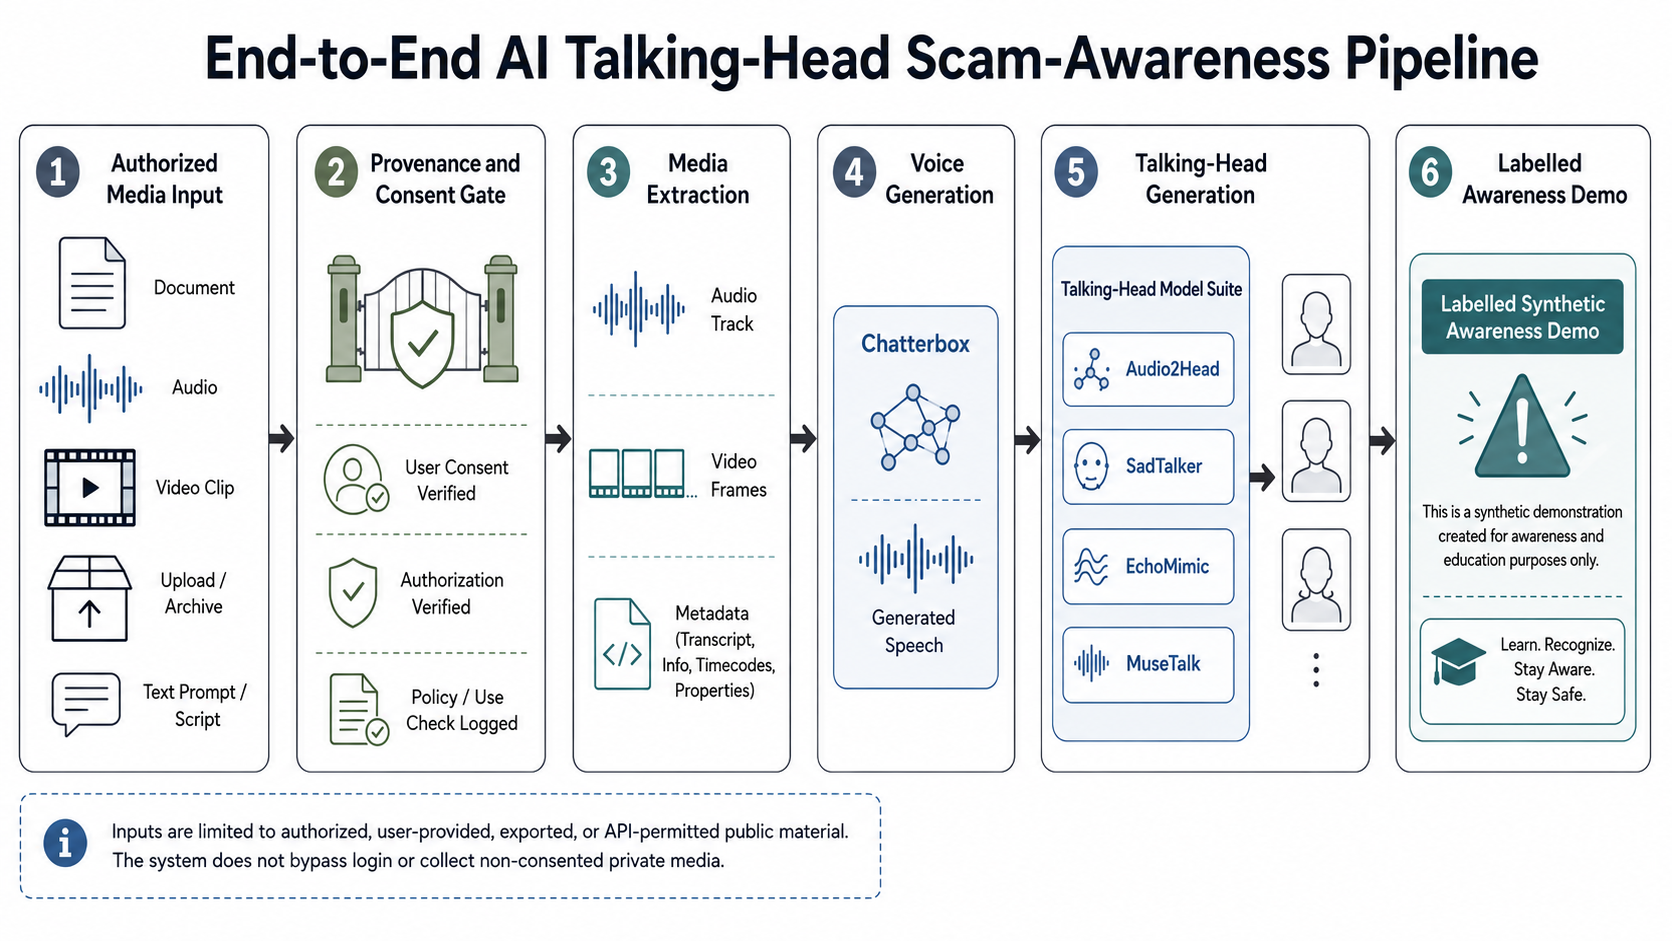
\includegraphics[width=0.98\textwidth]{figures/pipeline_gptimage2.png}
\caption{End-to-end AI talking-head scam-awareness pipeline. The system accepts authorised images, audio/video, text prompts, and exported materials; records provenance and consent; extracts face, audio, and metadata; generates speech and talking-head video; and outputs a labelled synthetic awareness demo.}
\label{fig:pipeline}
\end{figure*}

\subsection{Social-media media collection}
The planned Facebook component will collect candidate face and voice material only through permitted routes: user-provided downloads, Facebook data export, or official/API-permitted public-page media where allowed. The system will not bypass login, scrape private profiles, or collect non-consented personal media. Each collected item will store provenance, media type, consent status, source link or export path, and whether it is suitable for face or voice extraction. This makes the system suitable for a prevention-focused demonstration rather than covert scraping.

\subsection{Preprocessing and quality screening}
The system will extract voice from uploaded audio/video using ffmpeg and prepare images using full-image, centre-crop, and automatic face-crop modes. It will also record source conditions that may affect reliability: face scale, eye distance, sharpness, pose proxy, mouth opening, and visible occlusion. These measurements are adapted from the source-condition stress idea used in the attached talking-head benchmark: average output quality can hide failures that occur only for difficult source images.

\subsection{Generation pipeline}
The speech module will generate target speech from text and a voice reference. The prototype uses Chatterbox for zero-shot voice generation. The talking-head component compares Audio2Head, SadTalker, EchoMimic, and MuseTalk. These models cover older audio-driven warping, 3DMM-conditioned animation, diffusion-style portrait animation, and latent-space inpainting. The WebUI deployment prioritises SadTalker and MuseTalk for interactive demonstration because they are most useful for showing the trade-off between whole-face motion and lip precision. The output is a labelled demonstration video for awareness and evaluation, not an undisclosed impersonation tool.

\subsection{Evaluation and analysis methodology}
Figure~\ref{fig:evaluation} shows the planned evaluation logic. The project will compare models and settings, measure output quality, identify failure cases, and translate findings into prevention strategies.

\begin{figure*}[t]
\centering
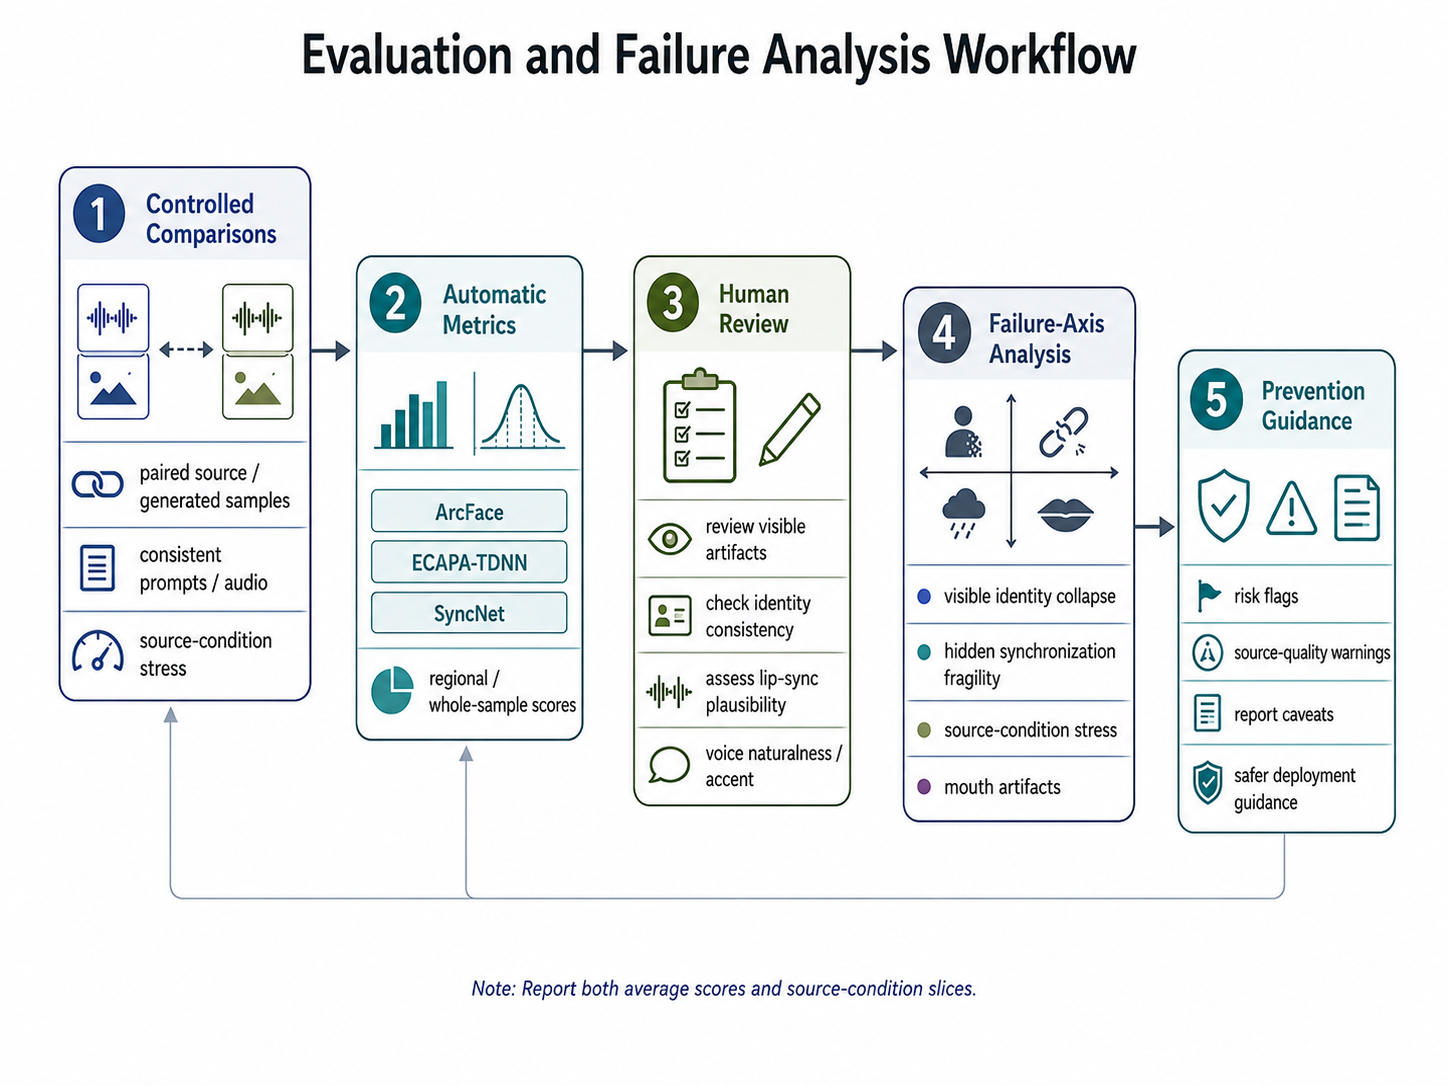
\includegraphics[width=0.92\textwidth]{figures/evaluation_gptimage2.png}
\caption{Evaluation and failure-analysis workflow. The system combines controlled model comparisons, automatic metrics, human review, failure-axis analysis, and prevention guidance, while reporting both average scores and source-condition slices.}
\label{fig:evaluation}
\end{figure*}

\section{Critical Functionalities}
The project is organised around the following critical functionalities. They turn the prototype from a simple generation demo into an evaluated awareness system.

\begin{table}[H]
\caption{Critical functionalities}
\label{tab:cf}
\centering
\scriptsize
\begin{tabular}{@{}p{0.13\columnwidth}p{0.81\columnwidth}@{}}
\toprule
\textbf{ID} & \textbf{Functionality} \\
\midrule
CF1 & Authorised image, audio/video, and text input with provenance and consent/use-status recording. \\
CF2 & Media extraction and preprocessing, including voice extraction, frame extraction, full-image mode, centre-crop mode, automatic face-crop mode, and source-quality checks. \\
CF3 & Voice generation from a text prompt and a voice reference, using Chatterbox as the working prototype backend. \\
CF4 & Talking-head video generation from the generated speech and source face image, using SadTalker and MuseTalk for the interactive WebUI path and Audio2Head/EchoMimic as comparison baselines. \\
CF5 & Controlled model comparison and metric collection, including ArcFace identity similarity, ECAPA-TDNN speaker similarity, SyncNet-style lip-sync measurement, and human review. \\
CF6 & Failure-case analysis that separates visible artefacts from hidden metric failures and maps each failure type to an improvement strategy. \\
CF7 & Safety and prevention support, including labelled synthetic outputs, source-quality warnings, documented collection limits, and user-facing scam-awareness guidance. \\
\bottomrule
\end{tabular}
\end{table}

\section{Research Questions}
\textbf{RQ1.} How can an authorised end-to-end pipeline transform facial images, voice/video references, and text prompts into labelled talking-head awareness demonstrations?

\textbf{RQ2.} How do Audio2Head, SadTalker, EchoMimic, and MuseTalk differ across identity preservation, lip synchronization, voice naturalness, visual realism, and source-condition robustness?

\textbf{RQ3.} Which provenance records, quality warnings, failure explanations, and user-facing guidance best support scam awareness and prevention?

\section{Comparison Experiments}
The project will include four comparison experiments. The model comparison covers Audio2Head, SadTalker, EchoMimic, and MuseTalk, and this four-generator evidence is used as the baseline for the awareness system.

\textbf{Backend comparison.} Audio2Head, SadTalker, EchoMimic, and MuseTalk are treated as the compared talking-head generators. They represent four mechanisms: audio-driven warping, 3DMM-conditioned animation, diffusion-style portrait animation, and latent-space inpainting. The expected trade-off is not one global winner, but different failure axes such as identity collapse, hidden lip-sync degradation, full-face motion quality, and mouth precision.

\textbf{Image preprocessing comparison.} Full-image, centre-crop, and automatic face-crop modes will be tested. This evaluates whether cropping improves focus or causes identity drift and mouth artefacts.

\textbf{Voice-reference comparison.} Short and longer clean voice references will be compared. This tests whether speaker similarity, accent retention, and naturalness improve with more suitable reference audio.

\textbf{Source-condition stress comparison.} Outputs will be sliced by source conditions such as small face scale, low eye distance, low sharpness, pose variation, and mouth opening. This uses the source-condition stress idea from the attached paper: a video can look plausible on average while failing under specific source conditions or on a hidden metric axis. In the four-model benchmark, Audio2Head exposes visible identity-collapse stress, while newer evaluated generators such as MuseTalk can remain identity-plausible but degrade on hidden synchronization axes.

\section{Evaluation Measures}
Table~\ref{tab:eval} summarises the measures. The project will not depend on one score, because talking-head realism is multi-dimensional.

\begin{table}[H]
\caption{Evaluation measures}
\label{tab:eval}
\centering
\scriptsize
\begin{tabular}{@{}p{0.24\columnwidth}p{0.70\columnwidth}@{}}
\toprule
\textbf{Aspect} & \textbf{Measure} \\
\midrule
Lip synchronization & SyncNet-style score where available and 1--5 human rating. \\
Identity preservation & ArcFace similarity between source image and generated frames. \\
Voice similarity & ECAPA-TDNN speaker similarity and human accent/naturalness rating. \\
Visual naturalness & Human rating of head motion, expression, mouth artefacts, and overall plausibility. \\
Robustness & Performance slices by face scale, sharpness, pose, mouth opening, crop mode, and backend. \\
Safety/usability & Provenance completeness, consent checks, warning visibility, and user questionnaire. \\
\bottomrule
\end{tabular}
\end{table}

\section{Failure Cases and Improvement Strategies}
Failure analysis is part of the project, not an afterthought. Expected failures include: accurate lips with a static head; natural head movement with weak mouth precision; mouth distortion from smiling or low-quality source images; identity drift after aggressive cropping; noisy references reducing voice similarity; and long text causing unnatural rhythm. The report will distinguish visible failures from hidden failures: a generated video may look plausible but still degrade in lip-sync or speaker similarity. Each failure will be linked to a mitigation such as changing the backend, adjusting crop mode, lowering expression scale, using cleaner 20--30 second reference audio, splitting long text, or warning the user when source quality is weak.

\section{Ethical Scope and Prevention Focus}
The project is framed as scam awareness and prevention. The system will not be deployed as a public impersonation service and will not remove disclosure or warning mechanisms. Facebook/social-media collection will be limited to authorised or permitted material. The final demonstration should be labelled as synthetic and used to explain risk, not to deceive real users. The countermeasure discussion will include user education, source verification, platform reporting, watermark/disclosure design, and warning signs of AI-generated identity-shifting content.

\section{Planned Deliverables}
The final submission will include: (1) a working WebUI demonstration; (2) a documented media collection and provenance workflow; (3) generated awareness examples; (4) comparison results using the four-generator baseline of Audio2Head, SadTalker, EchoMimic, and MuseTalk, plus crop-mode and voice-reference settings; (5) source-condition stress and failure-case analysis; and (6) a concise prevention discussion.

\section{Current Progress}
The main system-building work and comparison foundation have already been completed before November 2026. The remaining plan therefore focuses on human evaluation, voice-quality improvement, analysis, and final paper writing rather than additional core system construction.

\begin{table}[H]
\caption{Completed or established work before November 2026}
\label{tab:progress}
\centering
\scriptsize
\begin{tabular}{@{}p{0.22\columnwidth}p{0.72\columnwidth}@{}}
\toprule
\textbf{Area} & \textbf{Progress} \\
\midrule
Prototype & A local WebUI demonstration path has been built for uploading images, audio/video references, and text prompts, then generating talking-head demo outputs. \\
Voice module & A Chatterbox environment has been created and tested for generating speech from text and a voice reference. \\
Talking-head module & SadTalker and MuseTalk have been connected as working demonstration backends for face-and-mouth motion generation. \\
Media workflow & The authorised-media workflow has been set around user-provided files, user exports, or API-permitted public material, with provenance, source-quality, and consent/use-status records. \\
Comparison basis & Audio2Head, SadTalker, EchoMimic, and MuseTalk have been used as the four-generator comparison foundation, with crop-mode and source-condition stress analysis carried into this project. \\
Proposal assets & The project now has an IEEE-style proposal draft, a Chinese mirror version, and two diagrams covering the end-to-end pipeline and the evaluation workflow. \\
\bottomrule
\end{tabular}
\end{table}

\section{Remaining Timeline}
\begin{table}[H]
\caption{Remaining project timeline to February 2027}
\label{tab:timeline}
\centering
\scriptsize
\begin{tabular}{@{}p{0.22\columnwidth}p{0.72\columnwidth}@{}}
\toprule
\textbf{Period} & \textbf{Remaining work} \\
\midrule
Nov 2026 & Design and run the human evaluation: collect ratings on lip-sync plausibility, identity consistency, visual realism, voice naturalness, and scam-awareness usefulness. \\
Dec 2026 & Improve the voice-generation stage, focusing on cleaner reference audio, reference length, accent/naturalness, pacing, and selected re-generation of weak samples. \\
Jan 2027 & Analyse the human-review results and voice-improvement results; organise failure cases, prevention implications, and ethical discussion into the report. \\
Before Feb 2027 & Finalise the paper, figures, comparison tables, failure-case analysis, demo package, and submission materials. \\
\bottomrule
\end{tabular}
\end{table}

\section{Conclusion}
This project is suitable as an AI project because it combines implementation, model integration, controlled comparison, evaluation, and responsible-AI analysis. Its main value is not simply producing a realistic talking-head video, but using that capability to demonstrate social-media scam risk, expose technical failure conditions, and support prevention strategies.

\begin{thebibliography}{00}
\scriptsize
\bibitem{wav2lip} K. R. Prajwal, R. Mukhopadhyay, V. Namboodiri, and C. V. Jawahar, ``A Lip Sync Expert Is All You Need for Speech to Lip Generation In The Wild,'' arXiv:2008.10010, 2020.
\bibitem{audio2head} S. Wang, L. Li, Y. Ding, C. Fan, and X. Yu, ``Audio2Head: Audio-driven one-shot talking-head generation with natural head motion,'' in \emph{IJCAI}, 2021.
\bibitem{musetalk} Y. Zhang et al., ``MuseTalk: Real-Time High Quality Lip Synchronization with Latent Space Inpainting,'' arXiv:2410.10122, 2024.
\bibitem{sadtalker} W. Zhang et al., ``SadTalker: Learning Realistic 3D Motion Coefficients for Stylized Audio-Driven Single Image Talking Face Animation,'' arXiv:2211.12194, 2022.
\bibitem{echomimic} Z. Chen, J. Cao, Z. Chen, Y. Li, and C. Ma, ``EchoMimic: Lifelike Audio-Driven Portrait Animations through Editable Landmark Conditions,'' arXiv:2407.08136, 2024.
\bibitem{chatterbox} Resemble AI, ``Chatterbox TTS,'' GitHub repository, 2026. [Online]. Available: \url{https://github.com/resemble-ai/chatterbox}
\bibitem{ecapa} B. Desplanques, J. Thienpondt, and K. Demuynck, ``ECAPA-TDNN: Emphasized Channel Attention, Propagation and Aggregation in TDNN Based Speaker Verification,'' arXiv:2005.07143, 2020.
\bibitem{arcface} J. Deng et al., ``ArcFace: Additive Angular Margin Loss for Deep Face Recognition,'' arXiv:1801.07698, 2018.
\bibitem{syncnet} J. S. Chung and A. Zisserman, ``Out of Time: Automated Lip Sync in the Wild,'' in \emph{ACCV Workshops}, 2016.
\end{thebibliography}

\end{document}
